%%%%%%%%%%%%%%%%%%%%%%%%%%%%%%%%%%%%%%%%%%%%%%%%%%%%%%
\begin{frame}[plain, noframenumbering]
    \frametitle{Ejemplo: Coloides}
	\begin{center}
		\movie[showcontrols=true]
		{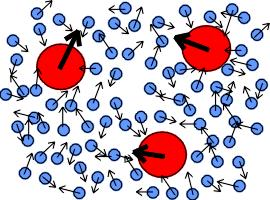
\includegraphics{./Imagenes/Introduccion/EsquemaColoides.png}}{Animacion16p.mpg}
	\end{center}
 \end{frame}
%---------------------------------------------------------------------------------------------------
%%%%%%%%%%%%%%%%%%%%%%%%%%%%%%%%%%%%%%%%%%%%%%%%%%%%%%%
\begin{frame}[plain, noframenumbering]
    \frametitle{Suspensiones Coloidales}
	 \begin{center}
		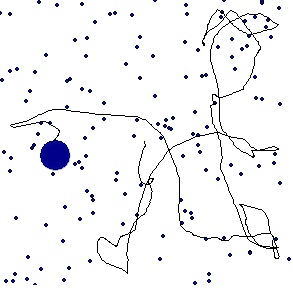
\includegraphics{./Imagenes/Introduccion/browngranular-foto2p.png}
	 \end{center}
\end{frame}
%%%%%%%%%%%%%%%%%%%%%%%%%%%%%%%%%%%%%%%%%%%%%%%%%%%%%%%%%%%%%%%%%%%%%%%%%%%%%%%%%%%%%
\tikzstyle{na} = [baseline=-.5ex]
\tikzstyle{every picture}+=[remember picture]
\everymath{\displaystyle}
%%%%%%%%%%%%%%%%%%%%%%%%%%%%%%%%%%%%%%%%%%%%%%%%%%
\begin{frame}[plain,noframenumbering]
  \frametitle{Formulación de Langevin}
  \begin{alertblock}{Ecuaciones de Movimiento}
    \begin{equation*}
      m\frac{d^2x}{dt^2}=
      \tikz[baseline]{
      \node[fill=blue!20,anchor=base] (t1)
      {$ -\gamma \frac{dx}{dt}$};
      }+
      \tikz[baseline]{
      \node[fill=green!20,anchor=base] (t2)
      {$\Gamma(t)$};
      }
    \end{equation*}
  \end{alertblock}
  \begin{columns}
    \column{.4\textwidth}
    \begin{itemize}
	\item <2-> $x=x(t)$:  posici\'on a tiempo $t$.
	\item <3-> Fuerza de fricci\'on, $\gamma=6\pi\eta a$,   $\eta$
	  viscosidad laminar 
	  $a$ radio  coloide.
	  \tikz[na] \node [coordinate] (n1) {};
	\item <4->$\Gamma(t)$ :
	  efecto estoc\'astico  
	  debido a las colisiones. \tikz[na] \node [coordinate] (n2) {};
    \end{itemize}
    \column{.6\textwidth}
  \end{columns} 
    \begin{tikzpicture}[overlay]
      \path [->]<3->  (n1) edge[bend right]  (t1);%
      \path [->]<4->  (n2) edge[bend right]  (t2);%
  \end{tikzpicture}
\end{frame}
%%%%%%%%%%%%%%%%%%%%%%%%%%%%%%%%%%%%%%%%%%%%%%%%%%%%%%%
\begin{bibunit}[apalike] 
 \begin{frame}[plain,noframenumbering]
   \begin{alertblock}{Al aplicar eliminación
	adiabática \cite{gardiner1985handbook}}
      \begin{equation*}
          \frac{dx}{dt}=\frac{1}{k_BT} D F+D^{\frac{1}{2}}\xi.
        \end{equation*}
    \end{alertblock}
  \begin{itemize}
      \item $x=x(t)$: posici\'on a tiempo $t$.
      \item $k_B,T$: $k_B$  constantes de  Boltzmann, $T$ temperatura,
      \item $F= -\frac{dU}{dx}$:  fuerza de la part\'icula inmersa en un potencial $U$,
      \item $D=\frac{k_BT}{6\pi\eta a}$: coeficiente de difusi\'on,
      \item $\xi$ : ruido blanco,\\
        $
         	\mathbb{E}(\xi(t)) =0, \quad
        	 \mathbb{E}(\xi(t)\xi(t'))=2\delta(t-t').
        $
   \end{itemize}
  \biblio{BibliografiaTesis}
\end{frame}
\end{bibunit}
%%%%%%%%%%%%%%%%%%%%%%%%%%%%%%%%%%%%%%%%%%%%%%%%%%%%%%%%%%%%%%%%%%%%%%%%%
\begin{frame}[plain,noframenumbering]
	\frametitle{Prop\'osito}
    \begin{block}
	{Resolvemos \quad $\frac{dx}{dt}=\frac{1}{k_BT} D F+D^{\frac{1}{2}}\xi.$}
	Para \textcolor{cyan}{entender} los mecanismos de \textcolor{cyan}{difusión}
	en una suspensión coloidal.
	\emph{Sin embargo, en la práctica \textcolor{red}{no se tiene solución analítica}.}
    \end{block}
  %\biblio{BibliografiaTesis}
\end{frame}
%%%%%%%%%%%%%%%%%%%%%%%%%%%%%%%%%%%%%%%%%%%%%%%%%%%%%%%%%%%%%%%%%%%%%%%%%%%%%%%%%%%%%%%%%%%%%%%
\definecolor{DarkSlateGrey}{HTML}{001B0C}
\definecolor{LightSteelBlue}{HTML}{B3D7F6}
\definecolor{DarkGray}{HTML}{394F50}
\definecolor{LightGoldenrodYellow}{HTML}{F8FDCB}
\setbeamercolor{color titulo caja}{fg=DarkSlateGrey,bg=LightSteelBlue} %%
\setbeamercolor{color cuerpo caja}{fg=DarkGray,bg=LightGoldenrodYellow}%
%==============================================================================================
\begin{frame}[plain, noframenumbering]
	\frametitle{Simulación de Dinámica Browniana}
	\tikzstyle{decision} = [diamond, draw, fill=yellow!20,
	text width=4.5em, text badly centered, node distance=4cm, inner sep=5pt]
	\tikzstyle{block} = [rectangle, draw, fill=blue!20,
	text width=5em, text centered, rounded corners, minimum height=4em]
	\tikzstyle{blockIm}= [rectangle, draw, fill=red!40,
	text width=6em, text centered, rounded corners, minimum height=4em]
	\tikzstyle{line} = [draw, -latex]
	\tikzstyle{cloud} = [draw, ellipse,fill=red!20, node distance=3cm,
	minimum height=2em]
	\begin{center}
		\begin{tikzpicture}[node distance = 2cm, auto]
		% Place nodes
		\node [block] (Init) {Inicializar};
		\node [block, below of=Init] (Fuerza) {Calculo de Fuerza};
		\node [decision, left of=Fuerza] (Serie) {Serie de Tiempo};
		\node [blockIm, below of=Fuerza] (Posiciones) {Posiciones};
		\node [block, left of=Posiciones,node distance=6cm] (Promedio){Promediar cantidades de interes};
		% Draw edges
		\path [line] (Init) -- (Fuerza);
		\path [line] (Fuerza) --(Posiciones);
		\path [line] (Posiciones)-|(Serie);
		\path [line] (Serie)--(Fuerza);
		\path [line] (Serie)-| (Promedio);
		\end{tikzpicture}
	\end{center}
\end{frame}
%%%%%%%%%%%%%%%%%%%%%%%%%%%%%%%%%%%%%%%%%%%%%%%%%%%%%%%%%%%%%%%%%%%%%%%%
\begin{bibunit}[apalike] 
\begin{frame}[plain,noframenumbering]
  \frametitle{Método convencional }
   \begin{exampleblock}{Euler-Mayurama (CBD)}
     \begin{align}
        Y_{j+1}^{(\alpha)}(h)=&
        	Y_{j}^{(\alpha)}+
        	\frac{D}{T}F_{j}^{(\alpha)}\Delta t+
        	R_{j}^{(\alpha)}\\        
      	\mathbb{E}
      		\left[
      			R_{j}^{(\alpha)}
        	\right]
        	=&0 \label{eqn:mediaEMc}\\
        \mathbb{E}
        \left[
        	R_{j}^{(\alpha)} R_{j}^{(\beta)}
		\right]
        	=&
        		2D h \delta_{ij}\delta_{\alpha \beta}
			&\alpha,\beta=x,y,z \label{eqn:CovEMc}
     \end{align}
    \end{exampleblock}
 	\begin{overlayarea}{\textwidth}{.4\textwidth}
	\only<+>{
  	\begin{columns}
		\column{.5\textwidth}
		\begin{itemize}
      		\item $Y_{j}^{(\alpha)}$: posición. 
      		\item $h:$ incremento temporal.
      		\item $F_{j}^{(\alpha)}:$ fuerza neta sobre la partícula $i$ en la dirección $\alpha$.
  		\end{itemize}
    	\column{.5\textwidth}
		\begin{itemize}
	        \item $R_{j}^{(\alpha)}:$ ruido blanco discreto, con  media y covarianza
		  	como en \eqref{eqn:mediaEMc} y \eqref{eqn:CovEMc}.
      		\item $D=\frac{k_B T}{\gamma}$: coeficiente de difusión de Stokes - Einstein
    	\end{itemize}
   	\end{columns}
	}
	\only<+>{
		\begin{columns}
		\column{.5\textwidth}
			\begin{itemize}
		  		\item Es explicito, barato y fácil de implementar.
		  	\end{itemize}
			\column{.5\textwidth}
			\begin{itemize}
			    \item Trabaja con un tamaño de \textcolor{red}{paso restrictivo}.
		  	\end{itemize}
	   	\end{columns}
	}
	\only<+->{
	\vspace*{-0.25cm}
		%\begin{exampleblock}{}
			Existen \textcolor{magenta}{varios} esquemas para discretizar la ecuación ya mencionada 
			\cite{branka1999blgorithms}.
	  		Sin embargo, \textcolor{cyan}{no} representan una \textcolor{cyan}{mejora significativa} 
	  		a la precisión respecto al coste computacional.
		%\end{exampleblock}
 	 }
 	 \vspace*{-.2cm}
	\only<+>{\biblio{BibliografiaTesis}}
	\end{overlayarea}
\end{frame}
\end{bibunit}
%%%%%%%%%%%%%%%%%%%%%%%%%%%%%%%%%%%%%%%%%%%%%%%%%%%%%%%%%%%%%%%%%%%%%%%%%%%%%%%%%%%%%%%%%%%%%%%%%%%%%
	\begin{frame}[plain,noframenumbering]
		\frametitle{EM diverge en sentido d\'ebil y fuerte.}    
		\begin{columns}
			\column{.4\textwidth}
				\begin{overlayarea}{\textwidth}{.5\textheight}
					Si el coeficiente de \textcolor{cyan}{deriva} o \textcolor{cyan}{difusión} 
					de una  EDE,
					\textcolor{cyan}{\emph{crece  más rápido que algo lineal}}, entonces el EM
					\textcolor{red}{diverge}.
					\only<2->{
						\\
						\textcolor{magenta}{Ejemplo:}
						\scalebox{.9}{\parbox{.5\linewidth}{%
						\begin{align*}
							dy(t) &= -10 \sign(y(t))|y(t)|^{\num{1.1}} dt + 4dW_t, \\
							y_0 &= 0, \quad t\in [0,10] \\
							&\approx \EX{|y(10)|}, \quad \num{e4}\text{ trayectorias }, \\
							& h=10/N, \quad N=\{1, 2,\dots,  50\}
						\end{align*}
						}
					}
				}
				\end{overlayarea}
			\column{.5\textwidth}
				\begin{overlayarea}{\textwidth}{.6\textheight}
					\only<3->{
						\vspace*{.12cm}
						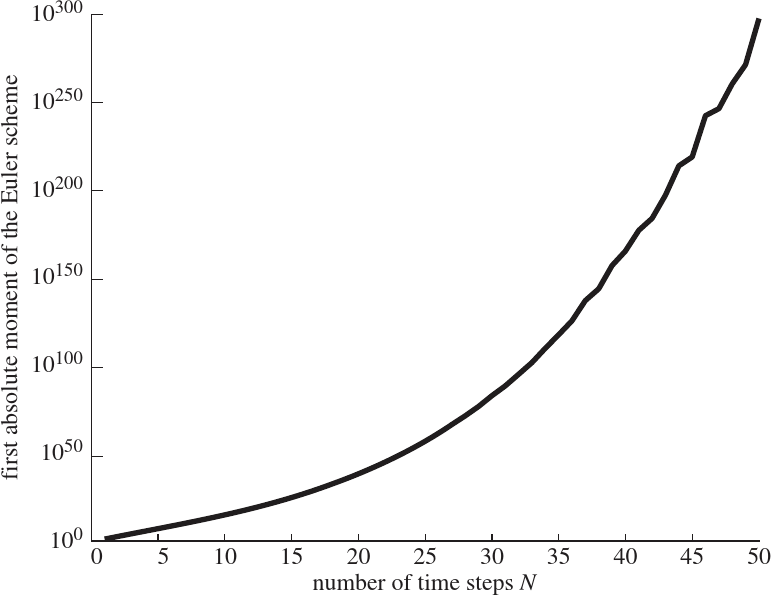
\includegraphics[width=\textwidth]
						{Imagenes/Introduccion/FirstMomenDivergenceEM}
					}
				\end{overlayarea}
		\end{columns}
		\begin{bibunit}[alpha]
			\nocite{Hutzenthaler2010}
			\biblio{PhdThesisBib.bib}
		\end{bibunit}
	\end{frame}
%%%%%%%%%%%%%%%%%%%%%%%%%%%%%%%%%%%%%%%%%%%%%%%%%%%%%%%%%%%%%%%%%%%%%%%%%%%%%%%%%%%%%%%%%%%%%%%%%%
	\begin{frame}[plain,noframenumbering]
		\frametitle{Modelos con Condiciones Local Lipschitz}    
		\begin{columns}
			\column{.3\textwidth}
				\begin{overlayarea}{\textwidth}{.3\textheight}
				  \begin{itemize}[<+-|alert@+>] 	
					  \item 
							  Biología
					  \item
						  Finanzas
					  \item
						  Física
					  \item
						  Química
					\end{itemize}
				\end{overlayarea}
			\column{.7\textwidth}
				\begin{overlayarea}{\textwidth}{.5\textheight}
					\begin{exampleblock}{
							\only<1>{Lotka Volterra}
							\only<2>{Henston}
							\only<3>{Langevin}
							\only<4>{Brusselator}
						}
						 \only<1>{
							\begin{align*}
								dX_t &= (\lambda X_t - k X_t Y_t ) dt +\sigma X_t dW_t\\
								dY_t &= (k X_t Y_t -mY_t) dt
							\end{align*}
						}
						\only<2>{
							\begin{align*}
								dS_t &= \mu S_t dt + \sqrt{V_t}S_t
									\left(
										\sqrt{1- \rho^2}dW^{(1)}_t
										+ \rho dW^{(2)}
									\right)\\
								dV_t &=
									\kappa (\lambda - V_t)dt +
									\theta \sqrt{V_t} dW^{(2)}_t
							\end{align*}
						}
						\only<3>{
							\begin{equation*}
								dX_t = -(\nabla U)(X_t)dt + \sqrt{2\epsilon}dW_t
							\end{equation*}
						}
						\only<4>{
							\begin{align*}
								dX_t =& 
									\left[
										\delta
										-(\alpha + 1) X_t +
										Y_t X_t^2
									\right] dt
									+ g_1(X_t) dW_t^{(1)} \\
								dY_t =&
									\left[
										\alpha X_t +
										Y_t X_t^2
									\right] dt
									+ g_2(X_t) dW_t^{(2)} \\
							\end{align*}
						}
					\end{exampleblock}
				\end{overlayarea}
		\end{columns}
		\begin{bibunit}
			\nocite{Hutzenthaler2015}
			\biblio{PhdThesisBib.bib}
		\end{bibunit}
		%
	\end{frame}
%%%%%%%%%%%%%%%%%%%%%%%%%%%%%%%%%%%%%%%%%%%%%%%%%%%%%%%%%%%%%%%%%%%%%%%%%%%%%%%%%%%%%%%%%%%%%%%%%%
\begin{frame}[plain,noframenumbering]
	\frametitle{Algúnas propuestas}    
	\begin{columns}
		\column{.3\textwidth}
			\begin{itemize}
				\item \structure<1-2>{\textbf{Impl\'icitos}:}
					\begin{itemize}[<+-| alert@+>]
%						\item
%							SSEM
						\item 
							$\theta$-BEM
						\item
							FBEM
					\end{itemize}
				\item \structure<3-5>{\textbf{Expl\'icitos}:}
					\begin{itemize}[<+-| alert@+>]
						\item 
							Tamed EM 
						\item
							Truncated
						\item
							Sabanis
					\end{itemize}
			\end{itemize}
		\column{.8\textwidth}
			\begin{overlayarea}{\textwidth}{.9\textheight}
%				\only<1>{
%					\begin{bibunit}[alpha]
%						\begin{block}{Split Step Euler Maruyama \nocite{Higham2002b}}
%							\begin{align*}
%								Y_k^{\star} &= Y_k + hf(Y^{\star}_k), \qquad Y_0 = y_0,\\
%								Y_{k+1}	&= Y_k^{\star} + g(Y_k^{\star})\Delta W_k 
%							\end{align*}
%						\end{block}
%						\biblio{PhdThesisBib.bib}
%						%\putbib
%					\end{bibunit}
%				}
				\only<1>{
					\begin{bibunit}[alpha]
						\begin{block}{$\theta$-Euler Maruyama \nocite{Mao2013}}
							\begin{align*}
								Y_{k+1} &= Y_k + h(1-\theta)f(Y_{k}) + 
								\theta f(Y_{k+1}) +
								g(Y_k)\Delta W_k,
								\\ & \theta \in [0,1].
							\end{align*}
						\end{block}
						\biblio{PhdThesisBib.bib}
					\end{bibunit}
				}
				\only<2>{
					\begin{bibunit}[alpha]
						\begin{block}{Forward-Backward Euler Maruyama \nocite{Mao2013}}
							\begin{align*}
								Y_{k} &= Y_{k-1} + h(1-\theta)f(Y_{k-1}) + 
									\theta f(Y_{k}) +
									g(Y_{k-1})\Delta W_{k-1}
									\\ 
								\widehat{Y}_{k+1} &= \widehat{Y_k} + hf(Y_{k}) + 
								g(Y_k)\Delta W_k,
								\qquad \theta \in [0,1].
							\end{align*}
						\end{block}
						\biblio{PhdThesisBib.bib}
					\end{bibunit}
				}
				\only<3>{
					\begin{bibunit}[alpha]
						\begin{block}{Tamed Euler Maruyama \nocite{Hutzenthaler2012a}}
							\begin{align*}
								Y_{k+1} &= Y_k + \frac{h f(Y_{k})}{1 +h \|f(Y_k)\|} + 
								g(Y_k)\Delta W_k
							\end{align*}
						\end{block}
						\biblio{PhdThesisBib.bib}
					\end{bibunit}
				}
				\only<4>{
					\begin{bibunit}[alpha]
						\begin{block}{Truncated Euler Maruyama \nocite{Mao2015}}
							\begin{align*}
								Y_{k+1} &= Y_k + f_{\Delta}(Y_k) h + g_{\Delta}(Y_k)\Delta_{k},\\
								f_{\Delta}(x)&:=
									\left(
										|x|\wedge \mu^{-1}(h(\Delta))\frac{x}{|x|}
									\right),\\
								g_{\Delta}(x)&:=
									\left(
										|x|\wedge \mu^{-1}(h(\Delta))\frac{x}{|x|}
									\right)
							\end{align*}
						\end{block}
						\biblio{PhdThesisBib.bib}
					\end{bibunit}
				}
				\only<5>{
					\begin{bibunit}[alpha]
						\begin{block}{Euler Maruyama with varying coefficients \nocite{Sabanis2015}}
							\begin{align*}
								Y_{k+1} &= Y_k + 
									\frac{h f(Y_{k}) + g(Y_k)\Delta W_k }
									{
										1 +k^{-\alpha} 
										\left(
											\|f(Y_k)\|
											+\|g(Y_k)\|
										\right)
									},
									\quad \alpha \in (0,1/2]  
							\end{align*}
						\end{block}
						\biblio{PhdThesisBib.bib}
					\end{bibunit}
				}
			\end{overlayarea}
	\end{columns}
\end{frame}
%%%%%%%%%%%%%%%%%%%%%%%%%%%%%%%%%%%%%%%%%%%%%%%%%%%%%%%%%%%%%%%%%%%%%%%%%%%%%%%%%%%%%%%%%%%%%%%%%
\begin{frame}[plain]
    \frametitle{Objetivo,noframenumbering}
    \begin{overlayarea}{\textwidth}{.5\textwidth}
    	\only<+>{
    		\begin{alertblock}{Objetivo}
			     M\'etodo 
			     \structure{\textbf{explicito}}, 
			     \structure{\textbf{barato}}, 
			     con condiciones 
			     \structure{\textbf{local Lipschitz}}
			      y 
			      \structure{\textbf{crecimiento super lineal}}.
			\end{alertblock}
		}
  \end{overlayarea}
\end{frame}
